\documentclass[conference]{IEEEtran}
\IEEEoverridecommandlockouts

\usepackage[utf8]{inputenc}
\usepackage[T1]{fontenc}
\usepackage[spanish,es-noindentfirst]{babel}
\usepackage{amsmath,amssymb}
\usepackage{graphicx}
\usepackage{tikz}
\usetikzlibrary{arrows.meta,positioning,fit,backgrounds,calc}
\usepackage{booktabs}
\usepackage{cite}
\usepackage{url}
\usepackage{xcolor}

\def\BibTeX{{\rm B\kern-.05em{\sc i\kern-.025em b}\kern-.08em
    T\kern-.1667em\lower.7ex\hbox{E}\kern-.125emX}}

\begin{document}

\title{CHASKI: NAVEGACIÓN AUTÓNOMA\\
EN EL LABERINTO}

\author{
\IEEEauthorblockN{Henry Tovar Landa\thanks{Grupo 4 (G4), Reto CapyTown Gran Prix, curso de Robótica, Universidad ESAN.}}
\IEEEauthorblockA{\textit{Universidad ESAN} \\ Lima, Perú \\ 24100514@ue.edu.pe}
\and
\IEEEauthorblockN{Julia Rojas Estrada}
\IEEEauthorblockA{\textit{Universidad ESAN} \\ Lima, Perú \\ 24100478@ue.edu.pe}
\and
\IEEEauthorblockN{Jordy Diaz Huanca}
\IEEEauthorblockA{\textit{Universidad ESAN} \\ Lima, Perú \\ 23101308@ue.edu.pe}
\and
\IEEEauthorblockN{Daniel León Condori}
\IEEEauthorblockA{\textit{Universidad ESAN} \\ Lima, Perú \\ 17100703@ue.edu.pe}
\and
\IEEEauthorblockN{Alex Perales Maldonado}
\IEEEauthorblockA{\textit{Universidad ESAN} \\ Lima, Perú \\ 22200107@ue.edu.pe}
}

\maketitle

\begin{abstract}
El Gran Prix CapyTown ``El Laberinto del Chaski'' plantea el desarrollo de un sistema de navegación autónoma capaz de recorrer un laberinto, respetar señales de tránsito y evitar obstáculos mediante percepción y control en tiempo real. Este trabajo presenta el diseño e implementación de la solución desarrollada por el Grupo 4 sobre una plataforma Yahboom Micro-ROS equipada con Raspberry Pi~5, LiDAR MS200 y cámara RGB, utilizando ROS~2 como entorno de integración.

La arquitectura propuesta se compone de tres nodos principales: \texttt{maze\_solver}, encargado de la navegación mediante una máquina de estados finitos y un controlador PD para el seguimiento de paredes; \texttt{pare\_detector}, responsable de la detección de señales PARE mediante segmentación en el espacio HSV y validación geométrica; y \texttt{box\_detector}, utilizado para la detección y evasión de obstáculos.

El sistema integra la información proveniente del LiDAR y la cámara mediante una estrategia de arbitraje que prioriza la percepción visual para el reconocimiento de señales y el LiDAR para la navegación. Los resultados experimentales muestran un comportamiento estable en la navegación por pasillos, una detección confiable de señales PARE y el correcto funcionamiento de los módulos desarrollados sobre la pista física. Finalmente, se presentan las principales decisiones de diseño, las medidas de seguridad implementadas y el trabajo pendiente para la validación durante las pruebas oficiales de competencia.
\end{abstract}


\begin{IEEEkeywords}
navegación autónoma, robótica móvil, fusión sensorial, LiDAR, seguimiento de pared, máquina de estados finitos, segmentación HSV, ROS~2, CapyTown
\end{IEEEkeywords}

\section{Introducción}

El Qhapaq Ñan era el gran camino inca, una red de senderos que se bifurcaban entre montañas, con atajos, desvíos y caminos que no llevaban a ningún lado. El Gran Prix CapyTown retoma esa metáfora para el reto final del curso: un robot, al que llamamos ``Karpinchu Chaski'', debe cruzar un laberinto de tablas de MDF desde el tambo de partida hasta la huaca de llegada, eligiendo su propia ruta sin que nadie lo maneje. El camino, eso sí, tiene reglas: en algunas intersecciones hay una señal de PARE, y un buen chaski se detiene por completo antes de seguir. Ganar no es solo llegar rápido, también se exige encontrar el camino más corto, respetar cada PARE y no derribar ninguna pared.

En el fondo, el reto es un problema de fusión sensorial con arbitraje, es decir, combinar la información de dos sensores distintos y decidir cuál manda en cada momento. El LiDAR resuelve la navegación geométrica: ¿por dónde hay pasillo?, ¿dónde hay una esquina?, ¿estoy metido en un callejón sin salida? La cámara, en cambio, responde una pregunta que el LiDAR no puede contestar: ¿hay un cartel PARE en esta intersección? Y esa respuesta tiene que poder interrumpir la navegación geométrica aunque el pasillo esté físicamente despejado. El objetivo de este artículo es documentar, con el nivel de detalle técnico que se puede verificar directamente en el código fuente, la arquitectura, los algoritmos y las decisiones de diseño del sistema que implementó el Grupo 4 para este reto, junto con la evidencia experimental que recogimos durante las pruebas de validación sobre la pista física.

El resto del artículo se organiza así: la Sección~II describe los Retos Clasificatorios previos cuyos nodos reutilizamos de forma explícita (uno de los requisitos del reto es ``fusionar, no reprogramar percepción''). La Sección~III detalla la arquitectura propuesta: los nodos de ROS~2, la máquina de estados de navegación, la ley de control de seguimiento de pared, el algoritmo de detección de PARE y la regla de arbitraje entre cámara y LiDAR. La Sección~IV describe la configuración experimental (plataforma, pista, parámetros). La Sección~V reporta los resultados de validación funcional obtenidos hasta el momento. Las Secciones~VI y VII discuten las decisiones de diseño y cierran con las conclusiones y el trabajo pendiente antes de las corridas oficiales.

\section{Antecedentes: Retos Clasificatorios Reutilizados}

El reto pide explícitamente no escribir percepción nueva salvo la estrictamente necesaria, sino fusionar piezas que ya construimos y depuramos en retos anteriores del curso. Heredamos tres piezas de forma directa.

\subsection{Seguimiento de pared y censo de cajas (RC-4)}
El controlador de seguimiento de pared, la detección de intersección o apertura y la recuperación en callejón sin salida del nodo \texttt{maze\_solver} son una adaptación de \texttt{maze\_navigator.py}, que desarrollamos para el Reto Clasificatorio ``El Censo y el Guardián de las Cajas'' (RC-4). De ese mismo reto reutilizamos, sin modificar su algoritmo, el nodo \texttt{box\_detector}, que segmenta el \texttt{/scan} (la lectura cruda del LiDAR) en tramos continuos, identifica protuberancias de unos 20\,cm de ancho como cajas (``karpinchus'') y las censa evitando contarlas dos veces gracias a su posición en el mundo, calculada con la odometría, que es la estimación de dónde está el robot a partir de cuánto se han movido sus ruedas.

\subsection{Detección de señales por color (RC de visión)}
La pieza de percepción por cámara (\texttt{pare\_detector}) es nueva para este reto, ya que los Retos Clasificatorios anteriores del equipo usaban solamente el LiDAR. Sin embargo, reutiliza el mismo flujo de calibración HSV interactiva (sliders en vivo y la tecla \texttt{s} para guardar la configuración en un archivo YAML) que empleamos en el detector de carril/color del RC de visión, adaptado aquí a la geometría de un cartel en forma de octágono rojo en lugar de una franja de carril.

\subsection{Extracción de líneas por Split \& Merge}
El módulo \texttt{split\_merge.py} implementa el algoritmo clásico Split \& Merge sobre las lecturas del LiDAR para extraer segmentos de recta, es decir, las paredes. En el Gran Prix lo incorporamos de forma aditiva dentro de \texttt{maze\_solver} únicamente para registrar en el log cuántas líneas y cajas detecta cada $\sim$2\,s; no participa en ninguna decisión de la máquina de estados de navegación, que opera sobre sectores angulares simples del \texttt{/scan}. Lo conservamos por si se puede reutilizar en otro reto del curso centrado específicamente en Split \& Merge.

\section{Arquitectura del Sistema Propuesto}

\begin{figure}[t]
\centering
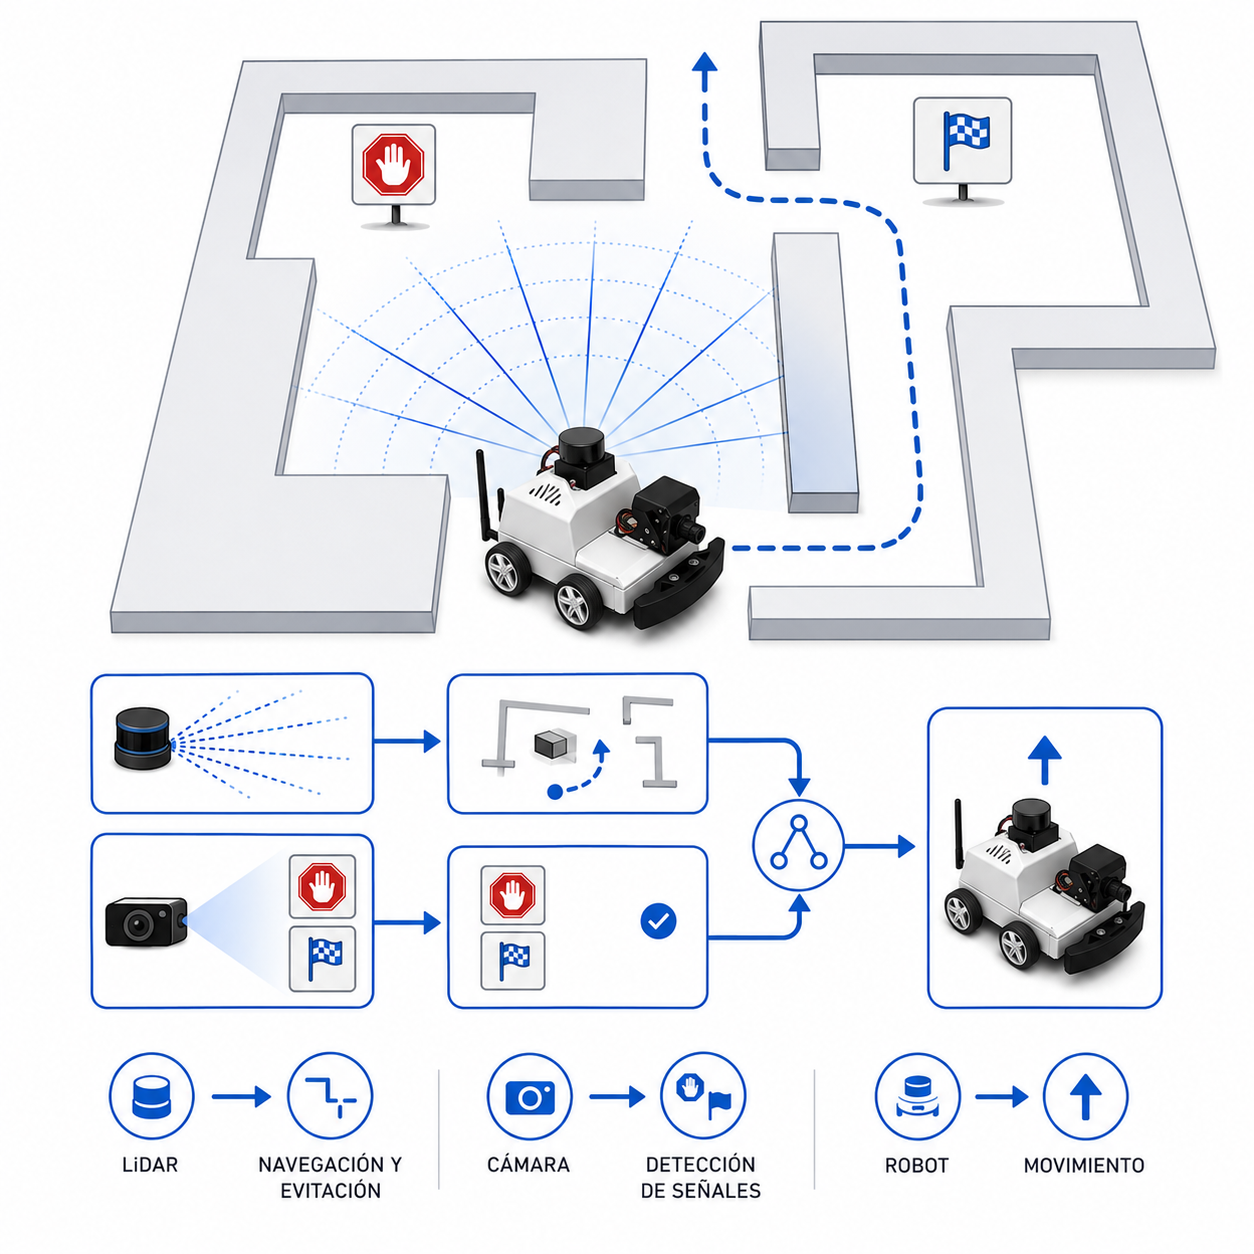
\includegraphics[width=0.95\linewidth]{figuras/fig_metodologia.png}
\caption{Metodología general: el LiDAR resuelve la navegación y evitación geométrica, la cámara resuelve la detección de señales (PARE/META), y ambas señales se arbitran antes de comandar el movimiento del robot.}
\label{fig:metodologia}
\end{figure}

La Fig.~\ref{fig:metodologia} resume esta metodología a alto nivel antes de entrar en el detalle por nodo.

\subsection{Visión general de nodos}
El sistema se implementa como el paquete de ROS~2 \cite{macenski2022ros2} \texttt{capytown\_granprix\_pkg} (\texttt{ament\_python}). ROS~2 es el framework de robótica que usamos para que los distintos programas del robot, llamados nodos, se comuniquen entre sí mediante tópicos, que son básicamente canales de mensajes: un nodo publica en un tópico y otro se suscribe a él para recibir esos mensajes. Lanzamos cinco nodos ejecutables con \texttt{launch/granprix.launch.py}: \texttt{maze\_solver}, \texttt{pare\_detector}, \texttt{box\_detector} (opcional, para la variante con karpinchus), \texttt{scan\_map\_viewer} (un visor en Tk, opcional) y \texttt{web\_dashboard} (un panel HTTP opcional en el puerto 8080). La Fig.~\ref{fig:arch} resume el flujo de tópicos entre nodos.

\begin{figure*}[t]
\centering
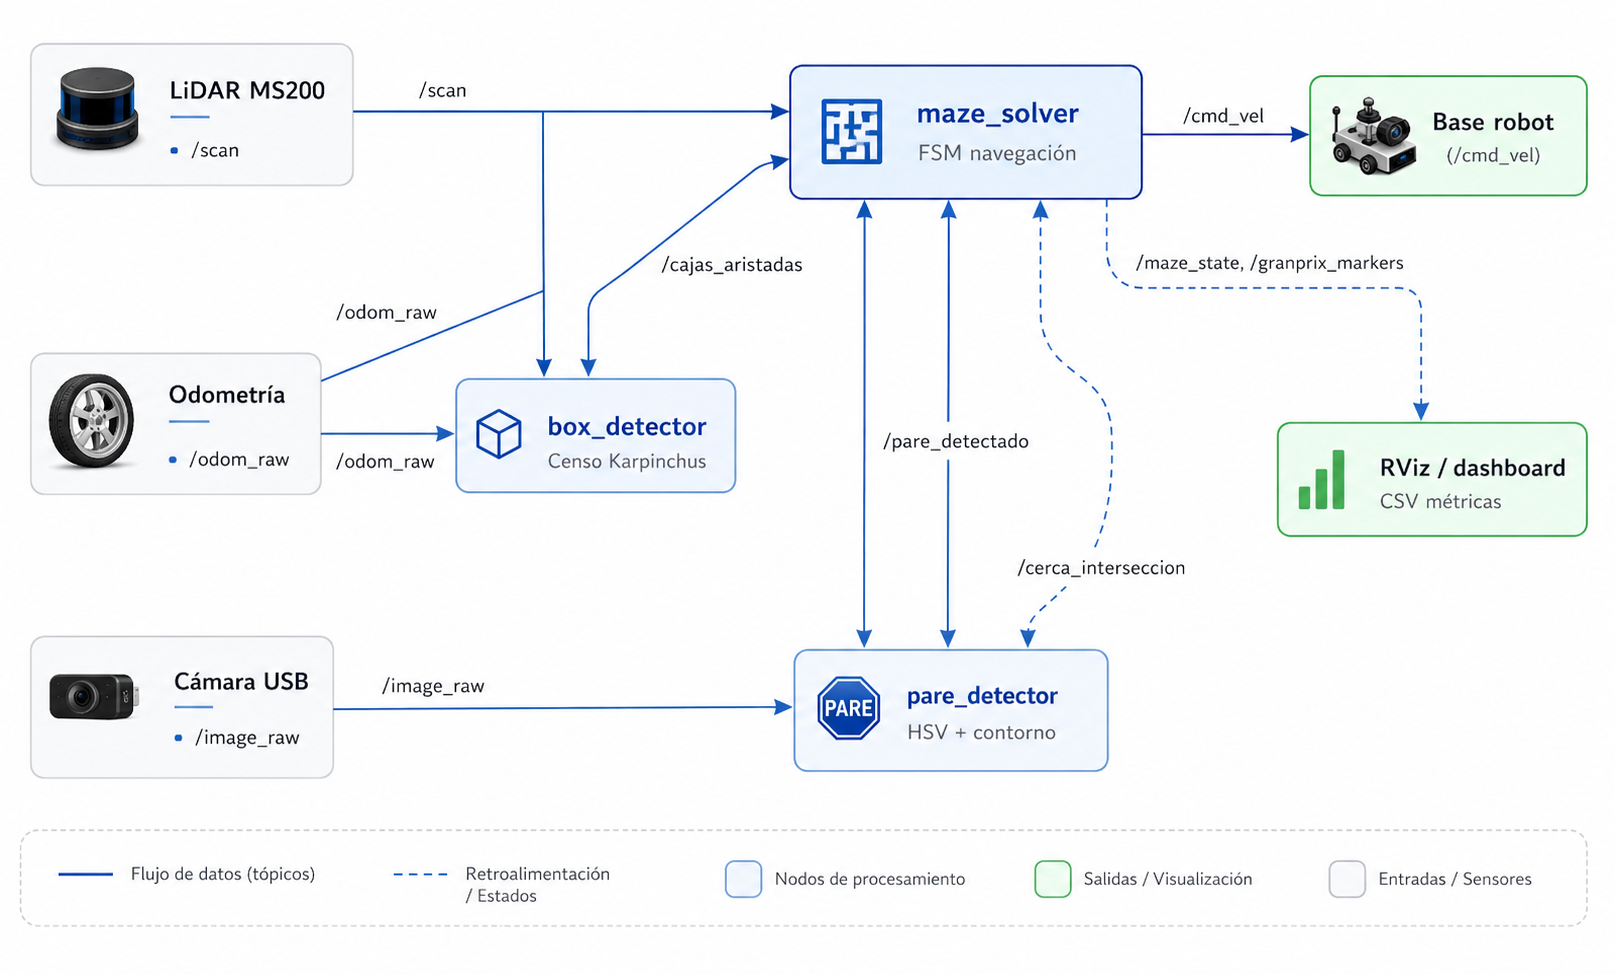
\includegraphics[width=0.92\linewidth]{figuras/fig_maquina_navegacion.png}
\caption{Arquitectura de nodos y tópicos ROS~2 del CapyTown Gran Prix. El LiDAR alimenta la geometría (\texttt{maze\_solver}, \texttt{box\_detector}); la cámara alimenta la semántica (\texttt{pare\_detector}); \texttt{maze\_solver} arbitra ambas señales (flujo discontinuo = retroalimentación/estado) y publica \texttt{/cmd\_vel}.}
\label{fig:arch}
\end{figure*}

\begin{figure}[t]
\centering
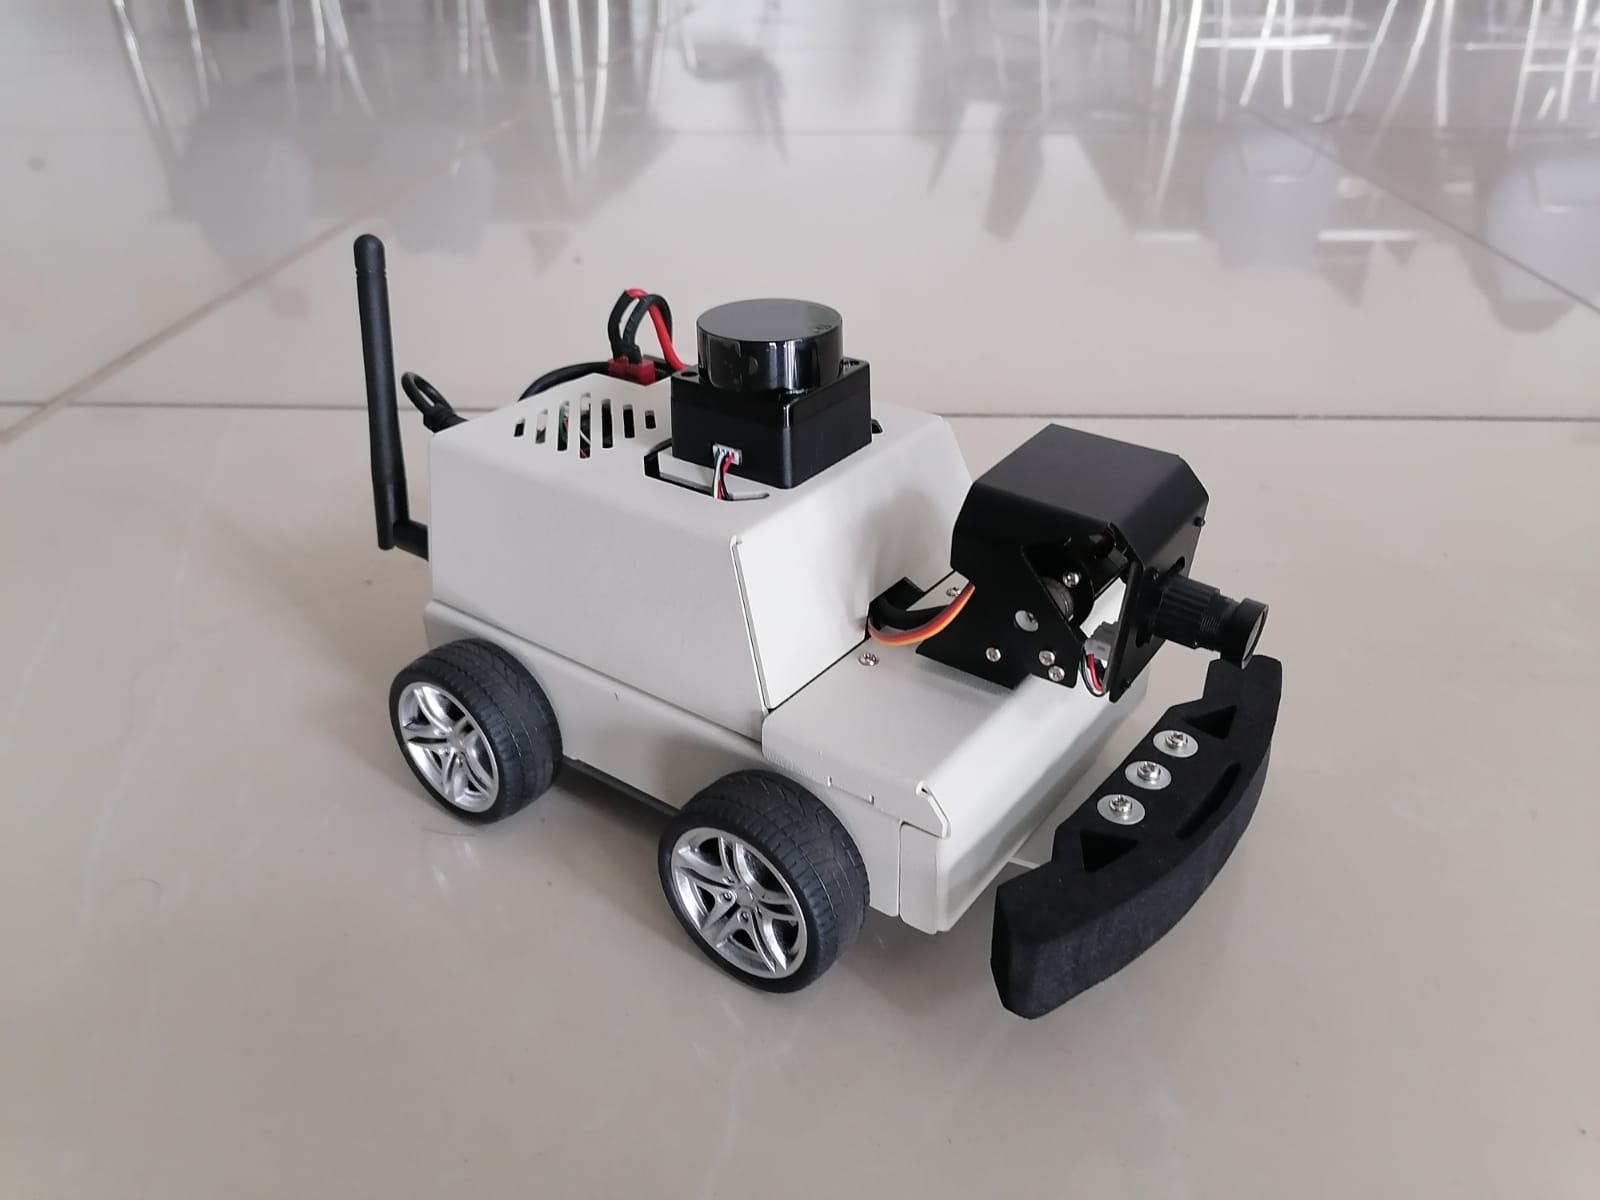
\includegraphics[width=0.85\linewidth]{figuras/fig_robot.jpeg}
\caption{Plataforma robótica utilizada: base Yahboom Micro-ROS con Raspberry Pi~5, LiDAR MS200 (torreta superior) y cámara sobre soporte pan orientable en el frente.}
\label{fig:robot}
\end{figure}

\subsection{Máquina de estados de navegación (\texttt{maze\_solver})}
La navegación geométrica se implementa como una máquina de estados finitos (FSM): un esquema en el que el robot solo puede estar en un estado a la vez, por ejemplo ``sigo la pared'' o ``estoy girando'', y salta de un estado a otro según lo que detecta. La implementamos como una función pura y testeable (\texttt{decide\_state}, independiente de ROS), con las siguientes transiciones, evaluadas en este orden de prioridad sobre las distancias mínimas de los sectores \texttt{front}, \texttt{left} y \texttt{right}:

\begin{enumerate}
  \item \textbf{Acorralado} (\texttt{front}, pared seguida y pared opuesta todas por debajo de \texttt{wall\_block}) $\rightarrow$ \textsc{Recover} (giro de $180^\circ$).
  \item \textbf{Apertura en la pared seguida} (\texttt{wall} $\geq$ \texttt{wall\_lost}) $\rightarrow$ \textsc{Turn\_Out} (gira hacia la pared para tomar la esquina, regla de la mano derecha/izquierda según \texttt{side}).
  \item \textbf{Frente bloqueado} (con histéresis y persistencia mínima \texttt{front\_block\_persist}) $\rightarrow$ \textsc{Turn\_In} (gira alejándose de la pared).
  \item En cualquier otro caso $\rightarrow$ \textsc{Follow\_Wall}.
\end{enumerate}

A estos cuatro estados geométricos se suma \textsc{Parar\_Pare} (forzado por la fusión con la cámara, que se explica en la Sección~III-G) y los estados terminales o de seguridad \textsc{Meta}, \textsc{Fault} y \textsc{Done}. Los giros de $90^\circ$/$180^\circ$ se ejecutan en lazo cerrado por odometría (\texttt{run\_turn}), no por tiempo: el robot gira hasta que el error angular respecto al \texttt{yaw} objetivo (la orientación del robot en el plano) cae bajo $4^\circ$, o hasta que el signo de ese error indica que ya se pasó del objetivo, lo que funciona como guarda contra el sobregiro, con un \emph{timeout} de seguridad de \texttt{turn\_timeout}$=6.0$\,s. Un detector de esquina alternativo (\texttt{corner\_pose\_aligned}) puede cortar el giro antes si la geometría del \texttt{/scan} (frente despejado, pared trasera visible, pared lateral seguida visible) ya corresponde a una pose de esquina correcta.

Un \emph{watchdog} anti-cascada (\texttt{turn\_in\_max\_accum\_deg}$=135^\circ$) evita que una secuencia de giros \textsc{Turn\_In} de $90^\circ$ sin avance real termine sumando $180^\circ$ efectivos, un bucle que detectamos en las pruebas de campo. Si el acumulado supera ese umbral, el robot retrocede en vez de volver a girar, y el acumulador solo se reinicia después de \texttt{turn\_in\_reset\_clear\_t}$=3.0$\,s con el frente sostenidamente despejado.

\subsection{Ley de control de seguimiento de pared}
El seguimiento de pared usa el esquema clásico de control proporcional-derivativo (PD): una ley de control que corrige el error actual (término proporcional) y también su tendencia a crecer o achicarse (término derivativo), aplicada aquí sobre el error lateral respecto a la pared seguida. Es el esquema típico en robots móviles con sensores de rango \cite{siegwart2011introduction,braunl2008embedded}:
\begin{equation}
e = d_{\text{obj}} - d_{\text{pared}}, \qquad
e_p = \begin{cases} 0 & |e| < \delta \\ e & \text{en otro caso} \end{cases}
\end{equation}
\begin{equation}
\omega = \mathrm{sgn}\;\big(k_p\, e_p + k_d\, \dot e\big), \qquad \dot e = \frac{e_k - e_{k-1}}{\Delta t}
\end{equation}
donde $\mathrm{sgn}=+1$ para seguimiento de pared derecha y $-1$ para pared izquierda, de forma que un error positivo (el robot está demasiado cerca) siempre lo haga girar alejándose de la pared que sigue. El término $\delta=$ \texttt{deadband}$=0.03$\,m evita que el robot ``surfee'' alrededor del punto de ajuste, y $k_p=0.70$, $k_d=1.60$ son las ganancias por defecto. La velocidad lineal se reduce de forma gradual entre \texttt{v\_min}$=0.06$ y \texttt{v\_max}$=0.18$\,m/s cuando el frente cae bajo \texttt{front\_slow}$=0.50$\,m. La distancia objetivo a la pared (\texttt{wall\_target}) y los umbrales de bloqueo frontal o lateral no son constantes fijas: se calculan a partir de la geometría física del robot (\texttt{robot\_width}$=0.16$\,m, \texttt{robot\_length}$=0.22$\,m) y de la separación deseada al borde (\texttt{wall\_clearance}$=0.12$\,m), de modo que el mismo nodo funcione sin recalibrarse sin importar el ancho real del pasillo el día de la prueba.

Sobre ese controlador base agregamos una corrección opcional por regresión de línea (\texttt{fit\_wall\_line}, activa por defecto con \texttt{line\_fit\_enabled}$=$\texttt{True}): en vez de leer la distancia lateral de un único sector, ajustamos por mínimos cuadrados una recta a todos los puntos del \texttt{/scan} dentro de una ventana angular de $70^\circ$ a $110^\circ$ respecto al lado seguido (\texttt{line\_window\_lo\_deg}/\texttt{line\_window\_hi\_deg}), con rechazo iterativo de valores atípicos (hasta \texttt{line\_outlier\_iter}$=3$ iteraciones, descartando puntos con residuo mayor a \texttt{line\_outlier\_residual\_m}$=0.03$\,m) para no dejar que los puntos de una esquina cercana sesguen el ajuste. Cuando hay al menos \texttt{line\_min\_points}$=6$ puntos válidos dentro de un rango corto (\texttt{line\_max\_range\_m}$=0.55$\,m), la corrección angular se calcula sumando el error de ángulo de la recta ajustada y el error de distancia perpendicular ($k_{\text{ángulo}}=1.2$, $k_{\text{distancia}}=0.70$), lo que resulta más robusto al ruido que un solo rayo; si no hay suficientes puntos (pasillo abierto, esquina), el nodo cae de vuelta automáticamente al controlador PD de sector descrito arriba. También agregamos dos factores de calibración de escala del odómetro, \texttt{factor\_dist\_odom} y \texttt{factor\_ang\_odom} (ambos en $1.0$ por defecto), para corregir un posible sesgo sistemático de \texttt{/odom\_raw} una vez medido en pista, sin tener que recalibrar el resto de los umbrales.

\subsection{Detección de intersecciones y callejones sin salida}
Los sectores de decisión se calculan con \texttt{sector\_robust}, que, a diferencia de tomar directamente el mínimo del sector, descarta primero los \texttt{sector\_drop}$=2$ rayos más cercanos antes de calcular el mínimo. Esto evita que un solo rayo con una lectura espuria, ruido típico del MS200, dispare una parada o un giro falso. El sector frontal cubre $\pm12^\circ$ y los sectores laterales van de $50^\circ$ a $100^\circ$ a cada lado. Una apertura (intersección o esquina) se detecta cuando la distancia a la pared seguida crece por encima de \texttt{wall\_lost}$=0.55$\,m (acotada de forma adaptativa a \texttt{corridor\_width}$-0.05$). Un callejón sin salida se detecta cuando el frente y ambas paredes laterales caen a la vez bajo \texttt{wall\_block}, y además exigimos que esa condición se mantenga durante \texttt{recover\_persist}$=1.0$\,s antes de disparar el giro de $180^\circ$, para no reaccionar a un roce momentáneo.

\subsection{Detección de PARE por cámara (\texttt{pare\_detector})}
El algoritmo es clásico y barato en cómputo, así que corre bien en el Raspberry Pi~5. Se apoya en OpenCV \cite{bradski2000opencv}, una librería estándar de visión por computador, y procesa cada cuadro de \texttt{/image\_raw} en cuatro pasos:
\begin{enumerate}
  \item Convertimos la imagen de BGR a HSV, un modelo de color donde el matiz, la saturación y el brillo están separados, lo que facilita segmentar por color sin que la iluminación arruine el resultado, y segmentamos el rojo con dos bandas, porque en OpenCV el tono rojo envuelve los extremos 0 y 179 del canal H: $H\in[0,10]$ y $H\in[170,179]$, ambas con $S\geq90$, $V\geq60$.
  \item Aplicamos una limpieza morfológica (una apertura seguida de un cierre, con un núcleo $5\times5$, para quitar ruido y rellenar huecos pequeños) y extraemos los contornos externos con el algoritmo de seguimiento de bordes de Suzuki y Abe (\texttt{cv2.findContours}) \cite{suzuki1985topological}.
  \item Filtramos el contorno candidato por su geometría: área mayor o igual a 350\,px$^2$, relación de aspecto ancho/alto entre $0.55$ y $1.8$ (para descartar franjas delgadas), \emph{extent} (el área dividida entre la caja delimitadora) de al menos $0.45$, y \emph{solidity} (el área dividida entre la del casco convexo) de al menos $0.75$. Este último filtro es el que descarta siluetas no convexas, como ropa o piel, que tienen entrantes y por eso bajan su \emph{solidity}, mientras que un octágono o rombo real es casi convexo.
  \item Aplicamos un \emph{debounce} temporal: solo publicamos \texttt{True} en \texttt{/pare\_detectado} si al menos el 60\,\% (\texttt{debounce\_ratio}$=0.6$) de los últimos 5 cuadros (\texttt{debounce\_frames}$=5$) tuvo una detección válida. Así evitamos que un falso positivo de un solo cuadro, por ejemplo un reflejo, dispare una parada.
\end{enumerate}
También implementamos la ``zona de atención'' que pide el reto: si \texttt{use\_attention\_gate}$=$\texttt{True}, la detección solo se evalúa mientras \texttt{maze\_solver} reporta, a través del tópico \texttt{/cerca\_interseccion}, que el robot se está acercando a una intersección. Esa condición se calcula como frente por debajo de \texttt{front\_slow} \emph{o} pared seguida por encima del 85\,\% de \texttt{wall\_lost}, y sirve para reducir falsos positivos en tramos rectos largos donde no puede haber un PARE. El nodo también publica \texttt{/pare/debug\_image}, una imagen con la forma roja real resaltada (no un rectángulo genérico) y la etiqueta ``PARE'', que se puede ver con \texttt{rqt\_image\_view} (Fig.~\ref{fig:pare_test} y Fig.~\ref{fig:pare_deteccion}).

\begin{figure}[t]
\centering
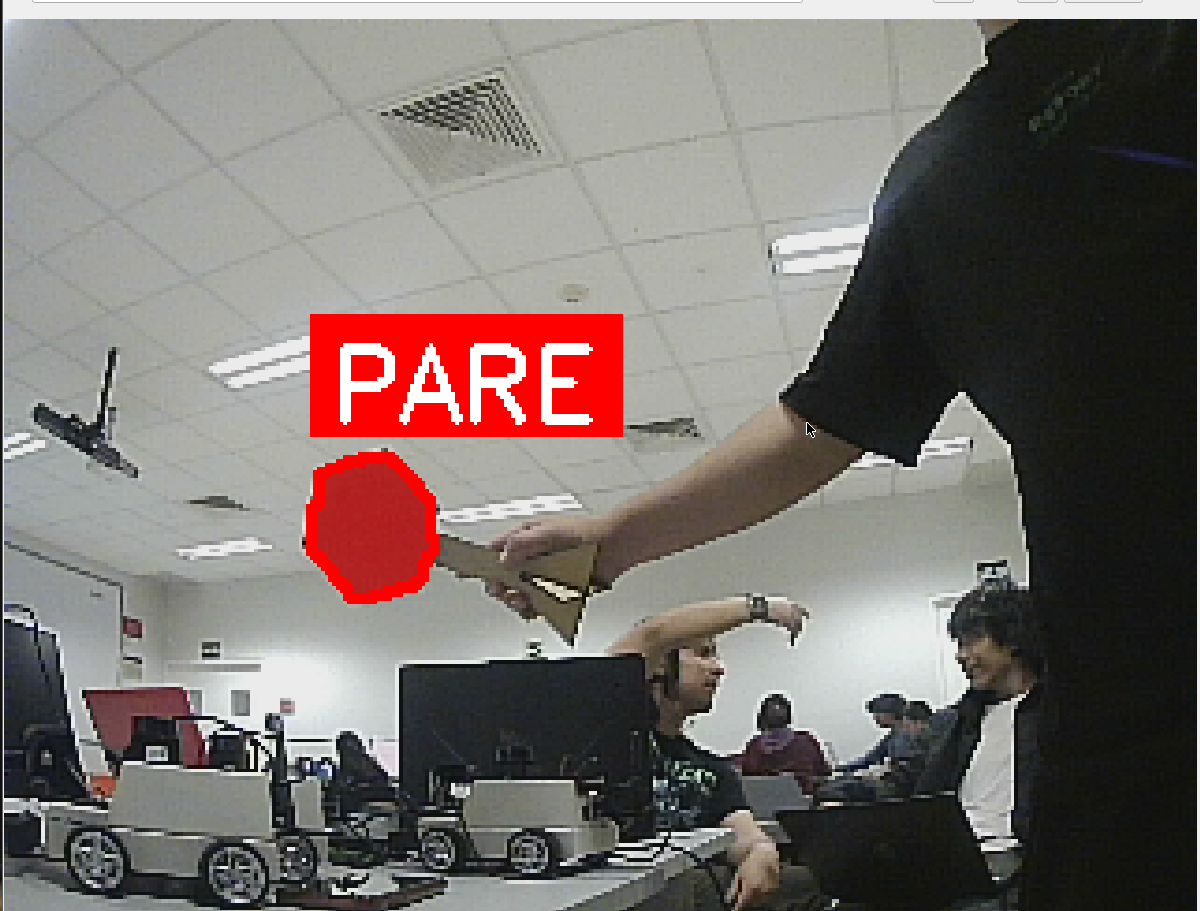
\includegraphics[width=0.85\linewidth]{figuras/fig_pare_test.png}
\caption{Prueba de calibración HSV: el algoritmo aísla la forma roja del cartel PARE sostenido frente a la cámara y superpone el contorno detectado (\texttt{/pare/debug\_image}).}
\label{fig:pare_test}
\end{figure}

\subsection{Censo y rodeo de karpinchus (\texttt{box\_detector})}
Para la variante opcional con obstáculos, \texttt{box\_detector} segmenta el \texttt{/scan} en tramos continuos (un salto de rango mayor a $0.12$\,m separa dos tramos), calcula el ancho físico de cada tramo multiplicando la distancia por el arco angular que cubre, y lo clasifica como caja si ese ancho cae en $0.20\pm0.08$\,m \emph{y} además sobresale al menos \texttt{MIN\_PROTRUSION}$=0.05$\,m respecto al fondo de la pared vecina. Cada caja detectada se proyecta a coordenadas del mundo usando la pose de \texttt{/odom\_raw}, y se descarta como duplicado si cae a menos de \texttt{BOX\_MERGE\_DIST}$=0.30$\,m de una caja ya censada. El conteo se publica en \texttt{/cajas\_avistadas} (que \texttt{maze\_solver} usa para el contador \texttt{karpinchus\_rodeados} de la rúbrica) y las posiciones en \texttt{/cajas\_avistadas\_pos} (\texttt{PoseArray}, para monitoreo). Dentro de \texttt{maze\_solver}, un obstáculo frontal localizado (su centro está más cerca que los hombros laterales del robot, \texttt{localized\_front\_obstacle}) dispara una sub-máquina de estados de esquive (\texttt{OUT}$\to$\texttt{PASS}$\to$\texttt{BACK}, o retoma el rumbo directamente) que se detiene \texttt{box\_stop\_wait\_t}$=3.0$\,s frente a la caja antes de rodearla, sin perder el rumbo previo ni saltarse un PARE pendiente.

\subsection{Fusión y arbitraje cámara--LiDAR}
La regla de arbitraje del reto la implementamos de forma literal y con prioridad absoluta, salvo por la emergencia de colisión. Si \texttt{/pare\_detectado} es verdadero y no estamos en el periodo de enfriamiento (\texttt{pare\_cooldown\_t}$=2.5$\,s desde el último PARE respetado, para no volver a dispararse sobre el mismo cartel), la FSM entra en \textsc{Parar\_Pare}, publica velocidad cero y se queda así exactamente \texttt{pare\_wait\_t}$=3.0$\,s, y al terminar incrementa el contador \texttt{pare\_respetados}. Todo esto ocurre sin importar lo que indiquen los sectores del LiDAR. Lo único que puede anteponerse es la guarda de emergencia por colisión inminente (\texttt{emerg\_dist}$=0.15$\,m), de forma que un PARE nunca termine provocando un choque. Esto materializa exactamente la regla que pide el reto: la cámara manda para detener, el LiDAR manda para moverse y centrar.

\subsection{Capas de seguridad}
El nodo implementa varias guardas independientes de la lógica de navegación: se detiene por completo si el \texttt{/scan} tiene más de \texttt{scan\_timeout}$=0.5$\,s de antigüedad, porque eso significaría estar manejando a ciegas, o si la odometría tiene más de \texttt{odom\_timeout}$=1.0$\,s, porque su pose ya estaría desactualizada. También hay un \emph{watchdog} de estancamiento posicional: si el robot pasa \texttt{stuck\_t}$=2.5$\,s sin avanzar al menos \texttt{stuck\_dpos}$=0.03$\,m, dispara una reversa de \texttt{recovery\_t}$=1.0$\,s. Por último, antes de intentar rotar en el sitio, el nodo comprueba que el pasillo sensado en vivo sea físicamente suficiente, es decir, al menos tan ancho como la diagonal del robot (aproximadamente $0.27$\,m), para no terminar en el estado \textsc{Fault} por un \emph{timeout} de giro en un pasillo demasiado angosto.

\subsection{Métricas y monitoreo}
Al llegar a META (dentro de un radio de \texttt{meta\_radius}$=0.35$\,m alrededor del punto \texttt{meta\_x}, \texttt{meta\_y} en el marco de \texttt{/odom\_raw}) o al cerrar el nodo, \texttt{maze\_solver} escribe una fila en \texttt{metricas\_granprix.csv} con exactamente las columnas que pide la rúbrica del reto: \texttt{ronda}, \texttt{llego\_meta}, \texttt{tiempo\_s}, \texttt{long\_ruta\_cm} (integrada a partir de la odometría, descartando saltos $>0.5$\,m como ruido), \texttt{long\_optima\_cm} (medida a mano sobre el plano), \texttt{eficiencia} (el cociente entre \texttt{long\_optima\_cm} y \texttt{long\_ruta\_cm}), \texttt{colisiones}, \texttt{pare\_reales}, \texttt{pare\_detectados}, \texttt{pare\_respetados}, \texttt{pare\_falsos}, \texttt{dead\_ends\_visitados} y \texttt{karpinchus\_rodeados} (Tabla~\ref{tab:metrics}). Los campos que no se pueden medir de forma automática, como \texttt{colisiones} y los falsos PARE, quedan marcados como pendientes de completar por revisión de video, tal como pide el propio reto. En paralelo, el nodo publica \texttt{/maze\_state} (un texto legible con el estado en vivo), marcadores de RViz en \texttt{/granprix\_markers} para cada intersección, PARE y META, y atiende \texttt{/dashboard\_pause}, que permite pausar el robot manualmente desde el panel web sin que pierda el estado de la FSM.

\begin{table}[t]
\centering
\caption{Columnas de \texttt{metricas\_granprix.csv} (implementadas en \texttt{maze\_solver.write\_metrics})}
\label{tab:metrics}
\small
\begin{tabular}{@{}ll@{}}
\toprule
\textbf{Campo} & \textbf{Origen} \\
\midrule
ronda, llego\_meta & parámetro / evento META \\
tiempo\_s & reloj interno desde 1\textsuperscript{er} \texttt{/odom} \\
long\_ruta\_cm & integración de \texttt{/odom\_raw} \\
long\_optima\_cm & medición manual sobre el plano \\
eficiencia & long\_optima\_cm / long\_ruta\_cm \\
colisiones, pare\_falsos & manual (video / \texttt{ros2 bag}) \\
pare\_reales & parámetro (conteo real en pista) \\
pare\_detectados, pare\_respetados & contadores de \texttt{on\_pare}/FSM \\
dead\_ends\_visitados & contador de eventos \textsc{Recover} \\
karpinchus\_rodeados & contador de sub-FSM de esquive \\
\bottomrule
\end{tabular}
\end{table}

\section{Configuración Experimental}

\subsection{Plataforma robótica y sensores}
El robot es una base Yahboom Micro-ROS sobre Raspberry Pi~5, con un LiDAR 2D MS200 ($\sim$10\,Hz) montado en una torreta y una cámara USB sobre un soporte pan orientable en el frente (Fig.~\ref{fig:robot}). El robot expone \texttt{/scan} (\texttt{sensor\_msgs/LaserScan}), \texttt{/odom\_raw} (\texttt{nav\_msgs/Odometry}, con una configuración de calidad de servicio \texttt{BEST\_EFFORT}/\texttt{VOLATILE} típica de los drivers embebidos, que en la práctica prioriza mensajes recientes sobre no perder ninguno) e \texttt{/image\_raw} (\texttt{sensor\_msgs/Image}), y recibe comandos de velocidad en \texttt{/cmd\_vel} (\texttt{geometry\_msgs/Twist}).

\subsection{Pista: el laberinto físico}
La pista se construyó con tablas de MDF de $30\times60$\,cm puestas de canto sobre una rejilla de $6\times4$ celdas de 60\,cm ($360\times240$\,cm en total), con la apertura de INICIO en el borde izquierdo y META en la esquina opuesta, varias rutas válidas y callejones sin salida puestos a propósito (Fig.~\ref{fig:laberinto}). Las señales PARE son carteles octagonales rojos sobre un soporte de madera, colocados a la altura del campo de visión de la cámara en algunas intersecciones (Fig.~\ref{fig:robot_laberinto}).

\begin{figure}[t]
\centering
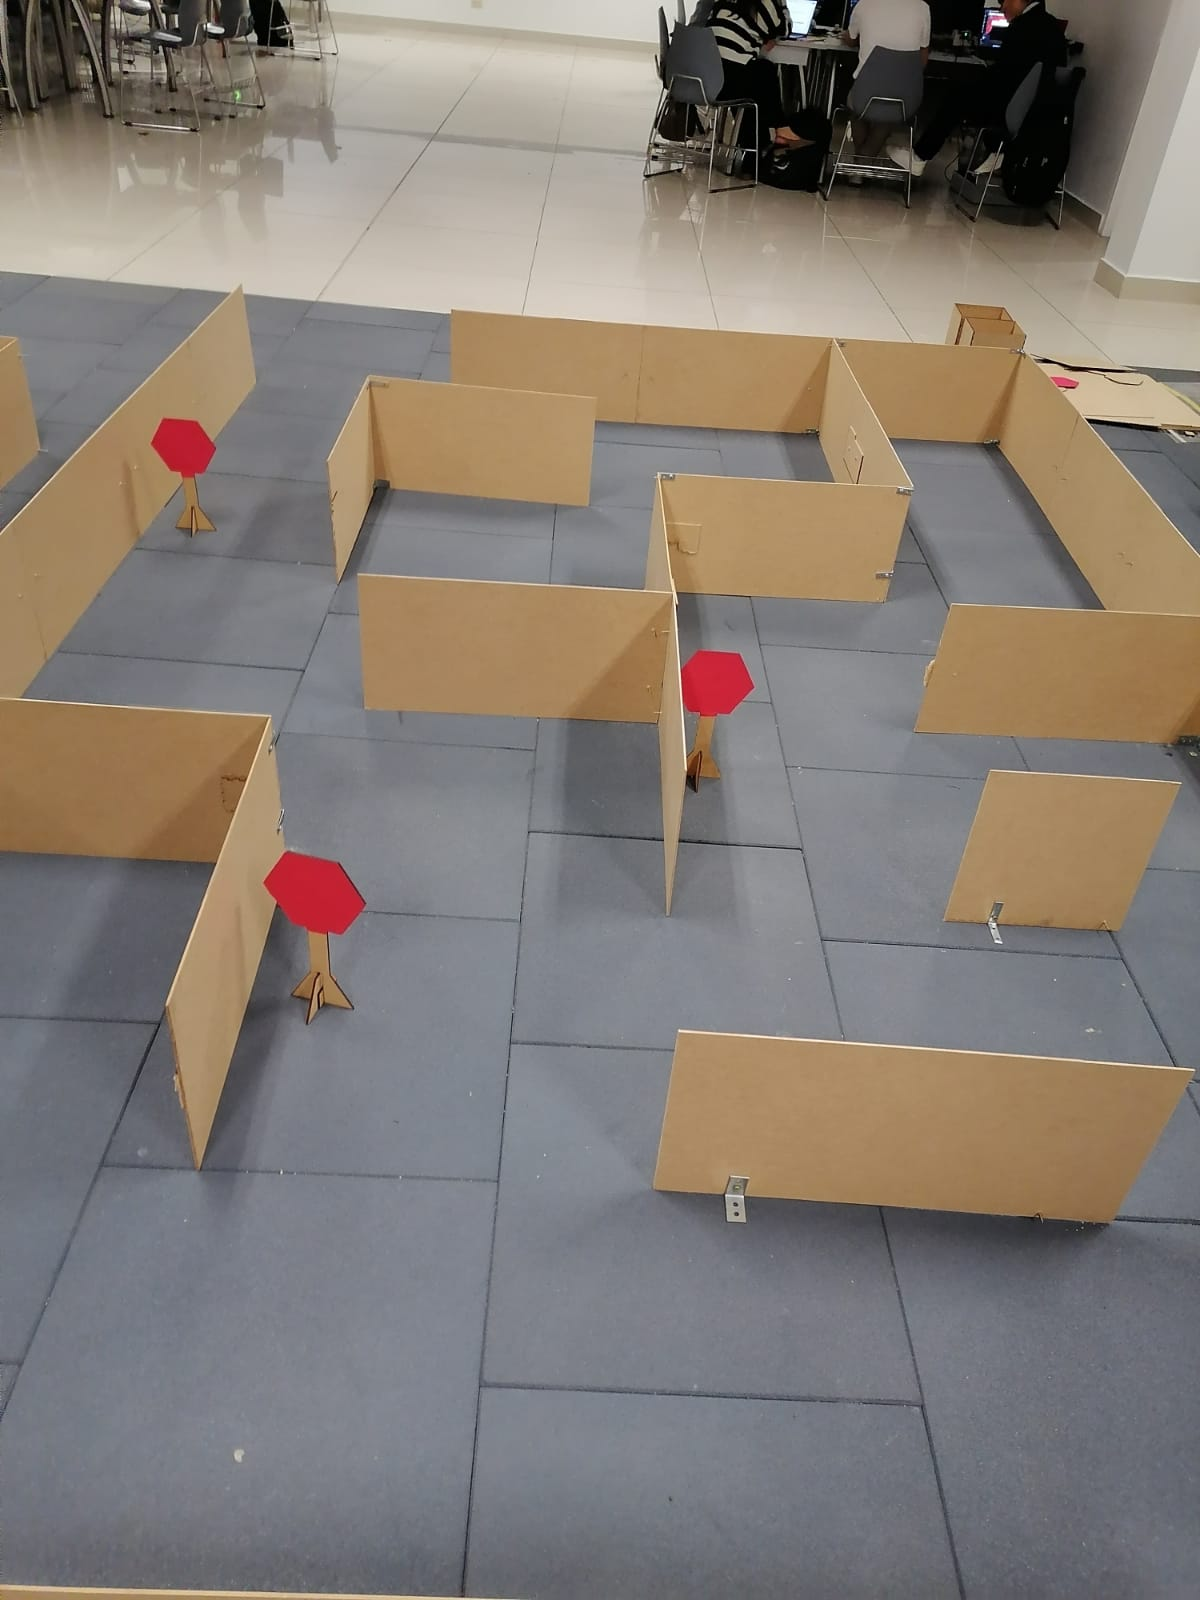
\includegraphics[width=0.95\linewidth]{figuras/fig_laberinto.jpeg}
\caption{Vista aérea de la pista construida: paredes de MDF de canto sobre rejilla $6\times4$ de 60\,cm, con dos señales PARE visibles en distintas intersecciones.}
\label{fig:laberinto}
\end{figure}

\subsection{Parámetros de ejecución}
La Tabla~\ref{tab:params} resume los parámetros de más alto nivel, que se pueden editar entre corridas desde \texttt{config/granprix\_params.yaml} sin tocar el código. Los umbrales de más bajo nivel del controlador (el PD, las aperturas, el callejón sin salida) ya vienen afinados en los \texttt{DEFAULTS} de \texttt{maze\_solver.py}, y se calculan de forma adaptativa a partir de la geometría del robot (Sección~III-C).

\begin{table}[t]
\centering
\caption{Parámetros de ejecución (\texttt{config/granprix\_params.yaml})}
\label{tab:params}
\small
\begin{tabular}{@{}lll@{}}
\toprule
\textbf{Nodo} & \textbf{Parámetro} & \textbf{Valor} \\
\midrule
maze\_solver & side (regla de mano) & right \\
maze\_solver & pare\_wait\_t / cooldown & 3.0\,s / 2.5\,s \\
maze\_solver & meta\_radius & 0.35\,m \\
maze\_solver & enable\_obstacle\_veer & true \\
pare\_detector & min\_area & 350\,px$^2$ \\
pare\_detector & aspect [lo, hi] & [0.55, 1.8] \\
pare\_detector & min\_extent & 0.45 \\
pare\_detector & debounce [frames, ratio] & [5, 0.6] \\
box\_detector & BOX\_SIZE $\pm$ TOL & 0.20 $\pm$ 0.08\,m \\
\bottomrule
\end{tabular}
\end{table}

\subsection{Protocolo de pruebas}
Antes de las corridas de competencia calibramos los rangos HSV directamente en la cancha, con el modo \texttt{--calibrar} de \texttt{pare\_detector.py} (sliders en vivo sobre el cartel real, bajo la iluminación del salón), y validamos cada nodo por separado: \texttt{pare\_detector} sosteniendo el cartel frente a la cámara (Fig.~\ref{fig:pare_test}), \texttt{maze\_solver} recorriendo tramos del laberinto en modo de seguimiento de pared, y \texttt{scan\_map\_viewer}/\texttt{web\_dashboard} para verificar en vivo cómo se clasifica el \texttt{/scan} entre PARED y CAJA, además de la trayectoria acumulada por odometría (Fig.~\ref{fig:scan_viewer}). El protocolo de competencia contempla dos rondas sobre la misma pista, reconfigurada entre una y otra: la Ronda~1 es de exploración, sin conocer el trazado, y la Ronda~2 es de \emph{time attack}, buscando la ruta más corta con cero colisiones y todos los PARE respetados.

\section{Resultados}

\subsection{Validación funcional por componente}
Las pruebas experimentales realizadas sobre la pista física permitieron verificar el funcionamiento de los principales módulos del sistema. La detección de señales PARE se mantuvo estable tanto durante la etapa de calibración (Fig.~\ref{fig:pare_test}) como en las pruebas realizadas dentro del laberinto (Fig.~\ref{fig:pare_deteccion}), donde el algoritmo identificó correctamente el contorno del cartel mediante la segmentación en el espacio HSV y los filtros geométricos implementados. El uso del criterio de solidity contribuyó a reducir falsas detecciones ocasionadas por objetos de color similar presentes en el entorno.

Asimismo, las pruebas de navegación evidenciaron que el controlador de seguimiento de pared mantuvo una trayectoria estable en los pasillos del laberinto. Como se observa en la Fig.~\ref{fig:robot_laberinto}, el robot logró desplazarse manteniendo una distancia lateral consistente respecto a la pared mientras la cámara supervisaba la detección de señales PARE en las intersecciones; el panel de monitoreo web (Fig.~\ref{fig:dashboard}) permitió verificar en vivo esa misma trayectoria y la segmentación del \texttt{/scan}. Estos resultados confirman el correcto funcionamiento de la estrategia de integración entre la información del LiDAR y la cámara durante la navegación.

\begin{figure}[t]
\centering
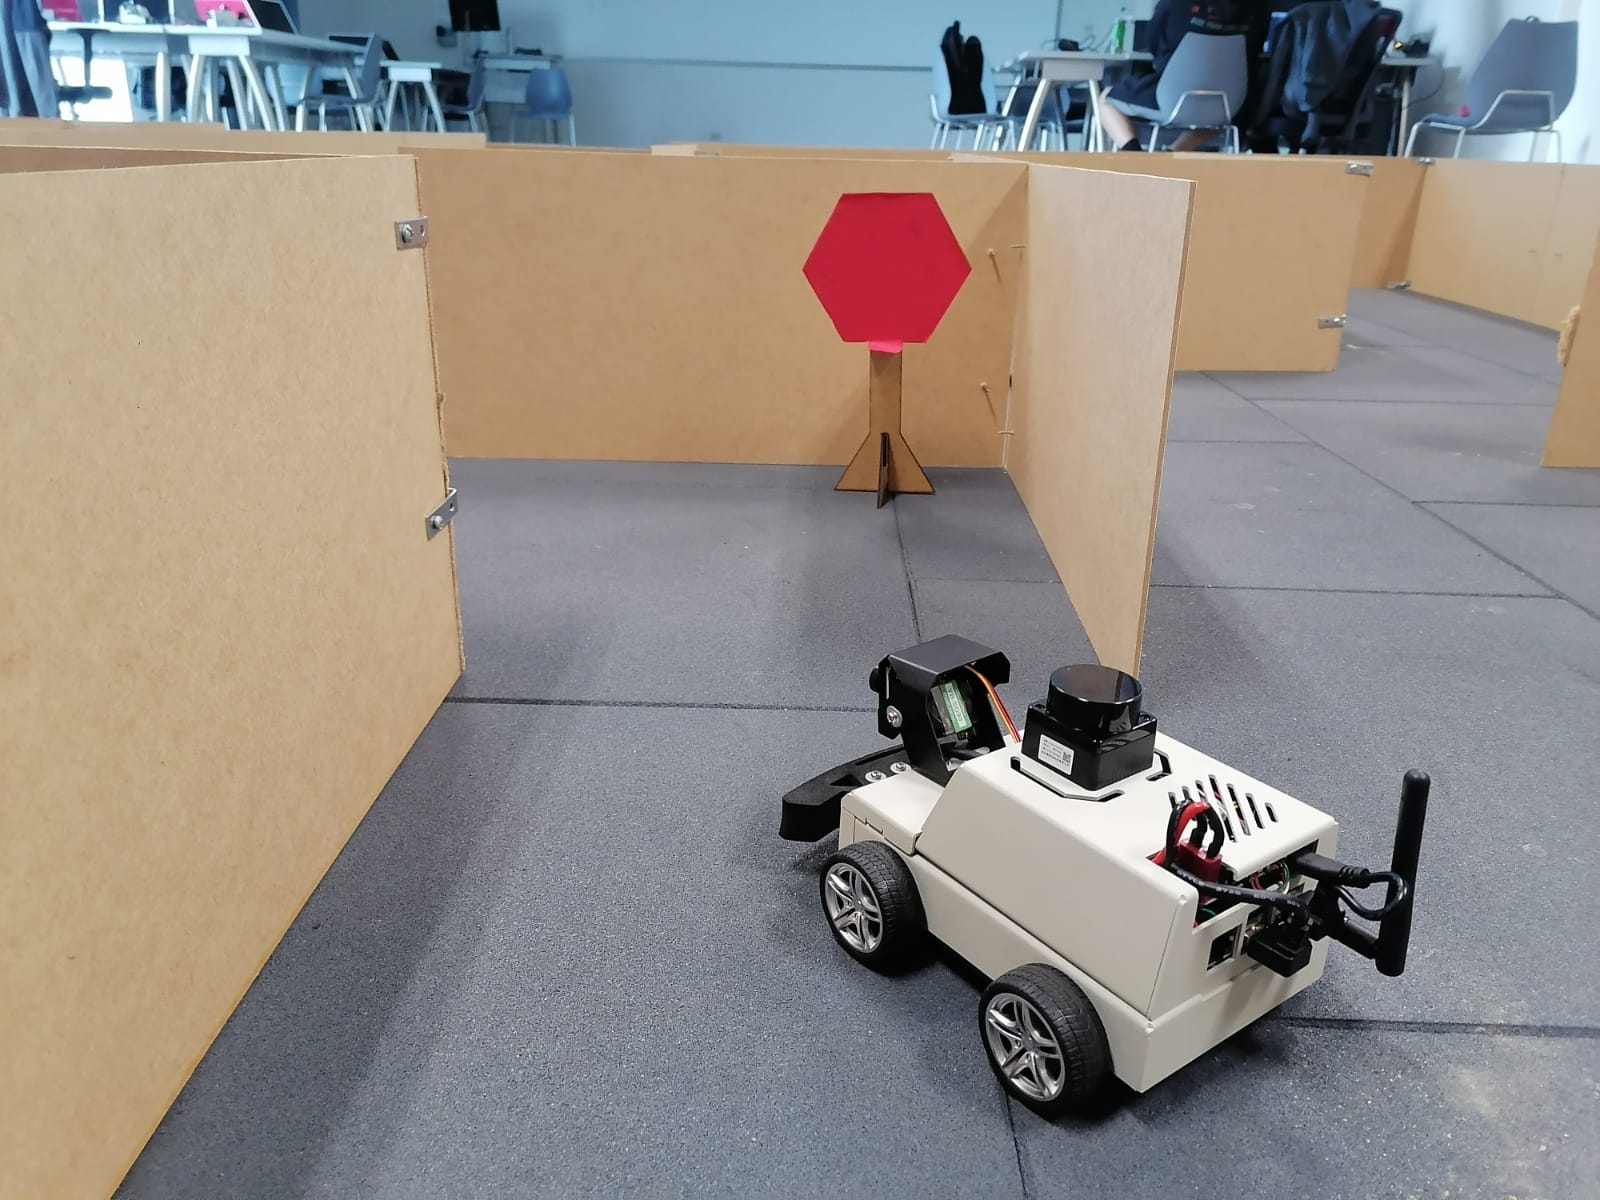
\includegraphics[width=0.85\linewidth]{figuras/fig_robot_laberinto.jpeg}
\caption{Robot aproximándose a una señal PARE dentro de un pasillo del laberinto durante el seguimiento de pared por LiDAR.}
\label{fig:robot_laberinto}
\end{figure}

\begin{figure}[t]
\centering
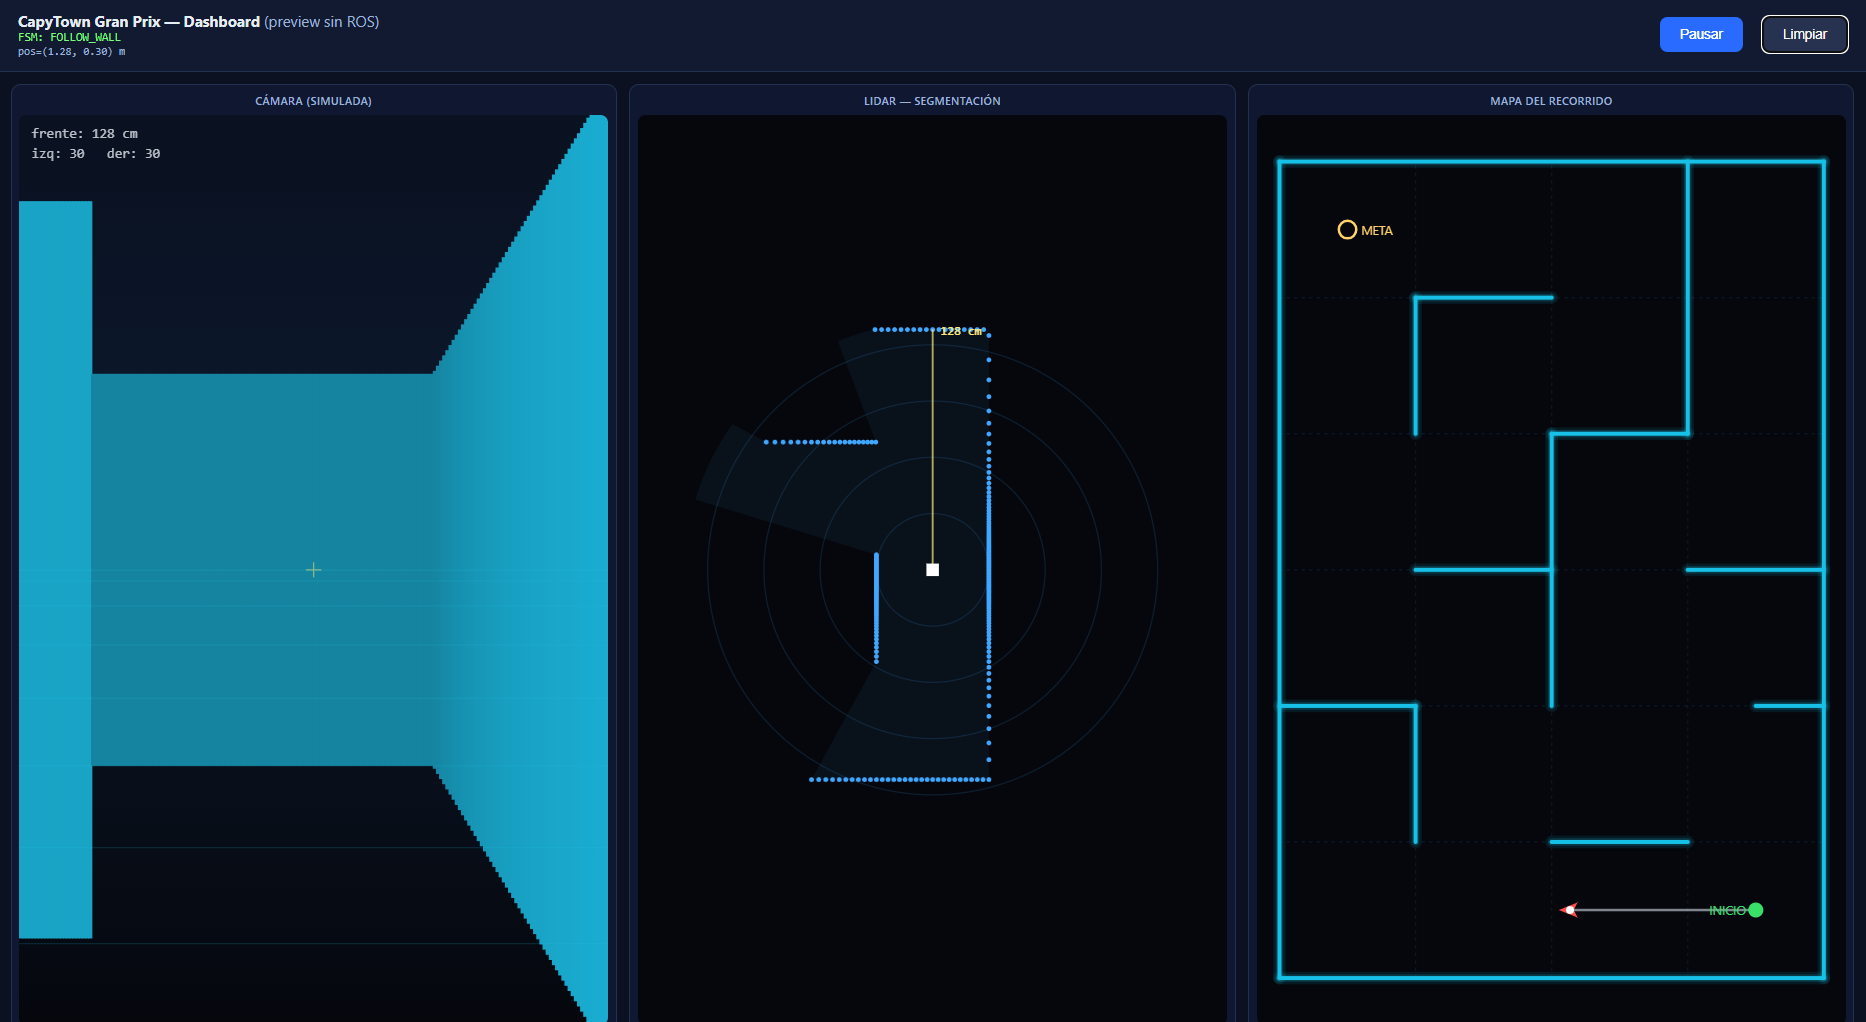
\includegraphics[width=0.95\linewidth]{figuras/fig_vista_camara_lidar.png}
\caption{Panel de monitoreo web (\texttt{web\_dashboard}): cámara, \texttt{/scan} segmentado y mapa del recorrido (INICIO/META) en una sola pestaña de navegador, con botón de pausa.}
\label{fig:dashboard}
\end{figure}

\begin{figure}[t]
\centering
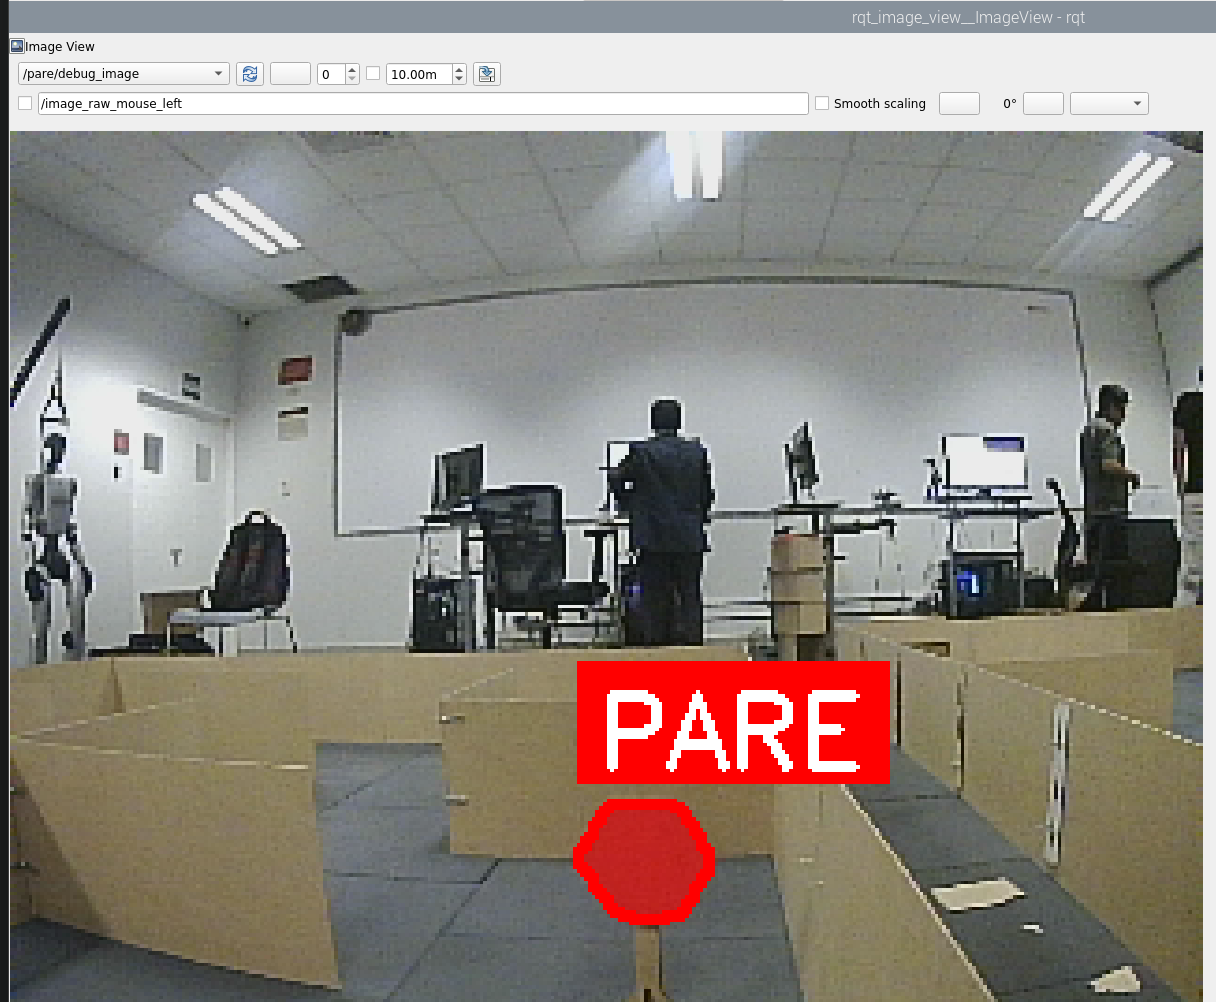
\includegraphics[width=0.85\linewidth]{figuras/fig_pare_deteccion.png}
\caption{Detección de PARE en vivo dentro del laberinto (\texttt{rqt\_image\_view} sobre \texttt{/pare/debug\_image}): el contorno real del cartel es resaltado y etiquetado.}
\label{fig:pare_deteccion}
\end{figure}

\begin{figure}[t]
\centering
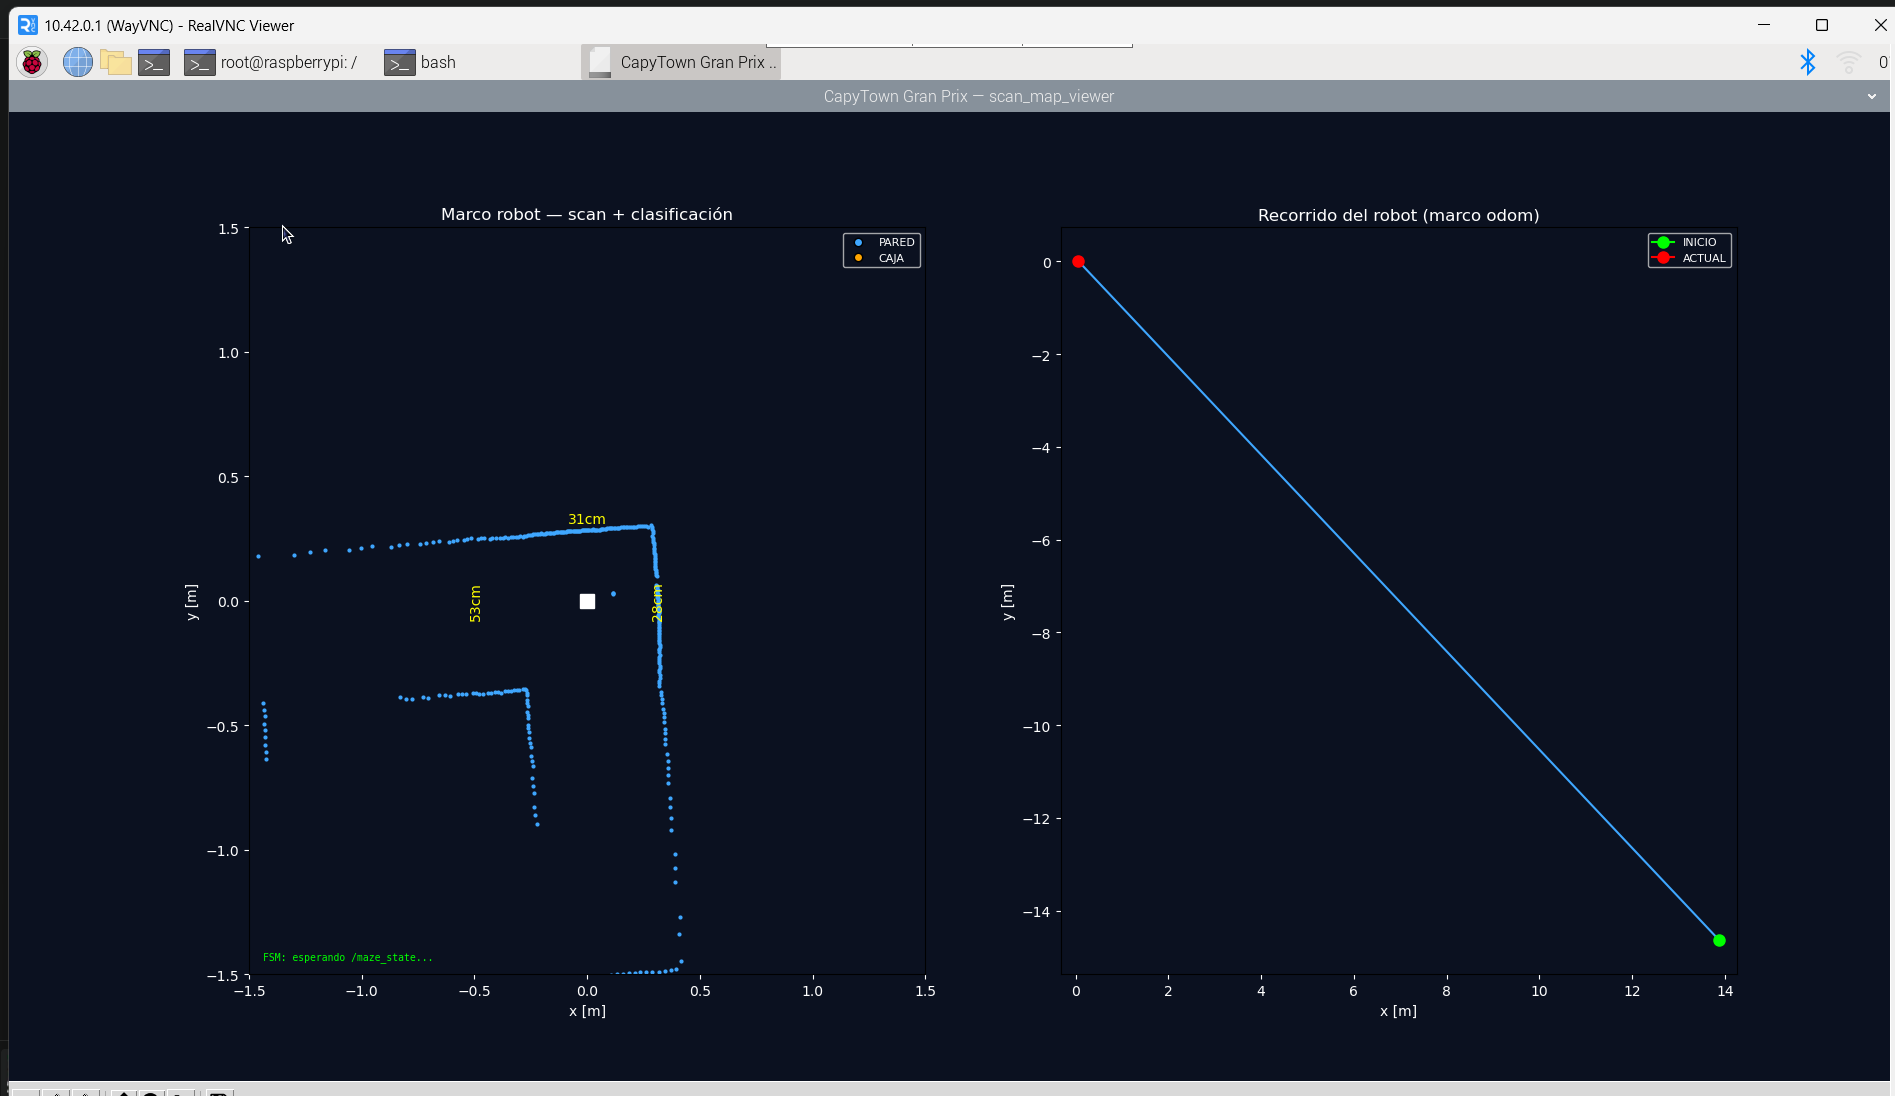
\includegraphics[width=0.95\linewidth]{figuras/fig_scan_viewer.png}
\caption{Panel de monitoreo (\texttt{scan\_map\_viewer}): a la izquierda, el \texttt{/scan} clasificado en PARED/CAJA en el marco del robot con las distancias de sector anotadas; a la derecha, la trayectoria acumulada por odometría desde INICIO.}
\label{fig:scan_viewer}
\end{figure}

\subsection{Estado de las métricas de competencia}
El esquema de \texttt{metricas\_granprix.csv} (Tabla~\ref{tab:metrics}) está implementado y verificado: escribe una fila completa tanto al llegar a META como al cerrar el nodo manualmente, así que ninguna corrida queda sin registrar. Sin embargo, al momento de escribir este artículo los parámetros \texttt{meta\_enabled}, \texttt{long\_optima\_cm} y \texttt{pare\_reales} de \texttt{config/granprix\_params.yaml} siguen en sus valores por defecto (\texttt{false}, 0.0 y 0, respectivamente), pendientes de medirse sobre la configuración real de la pista el día de cada corrida oficial, tal como indica el propio comentario del archivo de configuración. Por eso este artículo reporta evidencia de \textbf{validación funcional} de cada componente (detección de PARE, seguimiento de pared, censo de cajas, monitoreo en vivo), pero todavía no las métricas cuantitativas de las Rondas~1 y~2 (\texttt{tiempo\_s}, \texttt{eficiencia}, \texttt{colisiones}), que completaremos en las corridas de competencia con la pista y las señales PARE ya reconfiguradas.

\section{Discusión}

El sistema que implementamos es deliberadamente reactivo: sigue paredes y decide en cada intersección con la información local del \texttt{/scan}, en vez de construir primero un mapa de ocupación \cite{elfes1989occupancy} del laberinto completo y planificar sobre él con un algoritmo de búsqueda de camino mínimo como A* \cite{hart1968formal}. Un mapa de ocupación es, básicamente, una cuadrícula donde cada celda guarda qué tan probable es que esté ocupada por una pared, y A* es un algoritmo que busca el camino más corto sobre ese mapa. Elegimos no usarlos porque evitan la complejidad y el costo de cómputo de mantener un mapa consistente bajo el ruido de la odometría por \emph{dead-reckoning} \cite{thrun2005probabilistic}, es decir, estimar la posición solo a partir del movimiento de las ruedas, sin ninguna referencia externa que corrija el error acumulado, algo especialmente costoso en el Raspberry Pi~5. A cambio, no garantizamos en general la ruta más corta en la Ronda~2, salvo que la topología del laberinto nos favorezca. El diseño prioriza la robustez ante las condiciones reales de la pista física por encima de la optimalidad teórica.

Tres decisiones ilustran ese compromiso. La primera es anclar los umbrales de seguimiento de pared a la geometría del robot ($W$, $L$) en vez de a las dimensiones nominales del laberinto: así, el mismo nodo funciona sin recalibrarse aunque el ancho real del pasillo termine siendo distinto al del plano. La segunda es el filtro de \emph{solidity} en la detección de PARE, en vez de quedarnos solo con área y relación de aspecto. Lo agregamos específicamente porque siluetas convexas irregulares, como ropa o manos, pueden pasar un filtro de área y aspecto sin problema, pero casi nunca imitan la convexidad de un octágono real, así que este filtro reduce los falsos positivos sin necesidad de entrenar ningún clasificador. La tercera es que implementamos la regla ``la cámara manda para detener, el LiDAR manda para moverse'' como una interrupción de máxima prioridad en el bucle de control, antes que cualquier lógica de seguimiento de pared, y no como un estado más de la FSM geométrica. Lo hicimos así justamente para que la lógica de navegación nunca pueda ``competir'' con una parada de seguridad que la cámara ya confirmó.

La principal limitación por ahora es que el sistema todavía no ha corrido las dos rondas oficiales sobre la pista con la geometría y las señales PARE definitivas. Los umbrales de detección de intersección y de censo de cajas ya están afinados con datos de campo, pero la eficiencia de ruta y la tasa de PARE respetados sin falsos positivos, que son los dos criterios de mayor peso en la rúbrica de implementación, solo se pueden reportar con datos reales de esas corridas. Otra limitación que reconocemos en el propio código es que \texttt{colisiones} y \texttt{pare\_falsos} no son cosas que el robot pueda detectar por sí solo, así que dependen de revisar manualmente el video o el \texttt{ros2 bag} de cada corrida.

\section{Conclusión}

En este trabajo se desarrolló un sistema de navegación autónoma para el reto CapyTown Gran Prix, integrando sensores LiDAR y cámara RGB sobre una plataforma Yahboom Micro-ROS con ROS 2. La arquitectura implementada permitió dividir las funciones principales en módulos independientes para la navegación, la detección de señales PARE y la evasión de obstáculos, facilitando tanto el desarrollo como las pruebas de cada componente.

Las pruebas realizadas muestran que el sistema responde de manera estable durante el seguimiento de paredes y es capaz de detectar correctamente las señales PARE bajo las condiciones evaluadas. Asimismo, la integración de la información proveniente de la cámara y el LiDAR permitió mejorar la toma de decisiones durante la navegación dentro del laberinto.

Si bien el sistema cumple con los objetivos planteados para esta etapa del proyecto, aún queda pendiente validar su desempeño durante las corridas oficiales de competencia y analizar las métricas finales de tiempo, eficiencia y precisión. Como trabajo futuro, se plantea optimizar los parámetros de control y continuar realizando pruebas en diferentes condiciones para aumentar la robustez y confiabilidad del sistema.

\section*{Resumen para la sustentación (en lenguaje simple)}

El robot tiene que cruzar solo un laberinto de tableros, desde un punto de inicio hasta una meta, sin que nadie lo maneje. Para ``ver'' usa dos sensores que se complementan. El LiDAR es como un radar láser que gira y mide qué tan lejos está cada pared a su alrededor; con esos datos, el robot sabe si tiene pared a la derecha, si el frente está libre, si llegó a una esquina o si se metió en un callejón sin salida. La cámara, en cambio, no mide distancias: reconoce colores y formas, y su único trabajo es detectar el cartel rojo de PARE. Usamos dos sensores distintos porque cada uno resuelve un problema que el otro no puede: el LiDAR nunca podría ``leer'' un cartel, y la cámara sola no sabría seguir una pared con precisión. Por dentro, el robot funciona como una máquina de estados: en cada instante está en un solo modo (seguir pared, girar, recuperarse de un callejón sin salida, o parado en un PARE) y va saltando de un modo a otro según lo que detecta el LiDAR. Para seguir la pared usamos un control PD, que es simplemente una fórmula que corrige la trayectoria según qué tan lejos está de la distancia ideal a la pared, y también según qué tan rápido se está alejando o acercando, para que el giro sea suave y no oscile de un lado a otro. La regla más importante del sistema es el arbitraje entre los dos sensores: la cámara manda cuando hay que parar (si detecta un PARE, el robot se detiene tres segundos sí o sí, sin importar lo que diga el LiDAR), pero el LiDAR manda cuando hay que moverse y mantenerse centrado en el pasillo. Esa prioridad está programada como una interrupción que se revisa antes que cualquier otra decisión, para que las dos señales nunca puedan ``pelearse''. Además, el sistema tiene varias capas de seguridad por si algo falla: se detiene si los datos del sensor están muy viejos, si deja de avanzar por un rato, o si está a punto de chocar. Todo lo que el robot hace se guarda en un archivo de métricas, para poder evaluar después qué tan eficiente fue la ruta y cuántos PARE respetó. En resumen: el LiDAR le da al robot los ``ojos'' para moverse por el laberinto, la cámara le da el ``criterio'' para respetar las reglas del camino, y la máquina de estados es la que decide, en cada momento, a cuál de los dos hacerle caso.

\bibliographystyle{IEEEtran}
\bibliography{refs}

\end{document}
